\begin{figure*}
    \centering
    \subfigure[单个CMP道集. \label{fig:6a}]{
        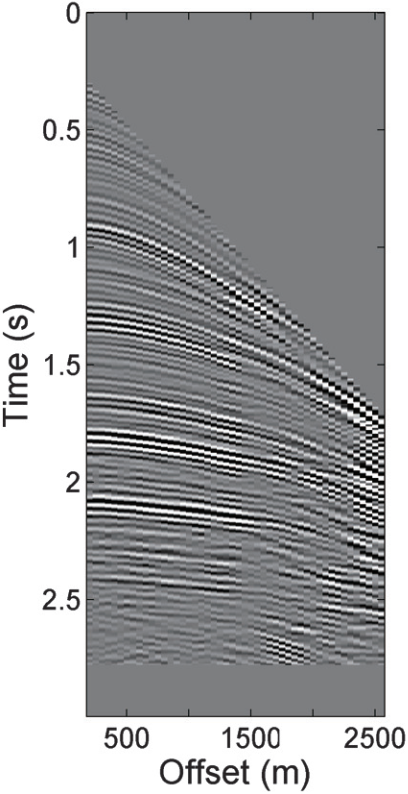
\includegraphics[scale=.33]{6a.png}
    }\ 
    \subfigure[由直方图函数计算出的近似聚类中心. \label{fig:6b}]{
        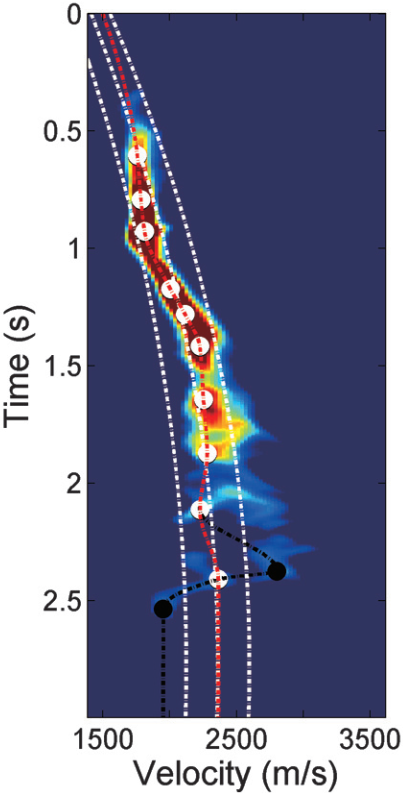
\includegraphics[scale=.33]{6b.png}
    }\ 
    \subfigure[NMO校正后的道集与自动估计叠加速度. \label{fig:6c}]{
        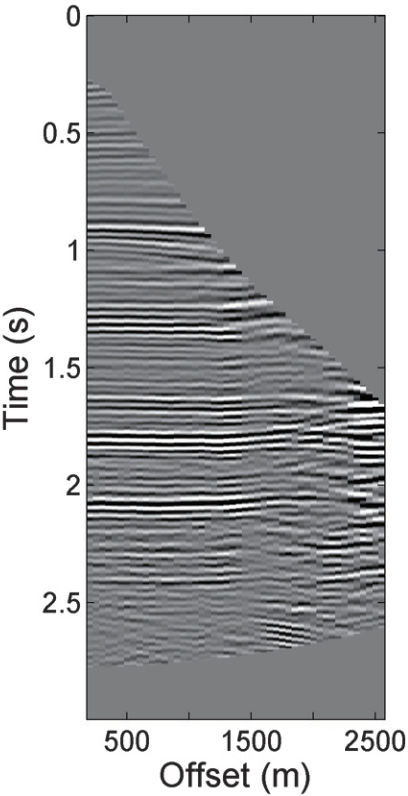
\includegraphics[scale=.33]{6c.png}
    }
    \caption{在Marmousi数据集中的单个CMP道集上提取的结点速度. 二阶多项式函数拟合的NMO速度和速度不确定度的上下界在 \ref{sub@fig:6b} 中用白色虚线标出. 超出速度不确定度的聚类速度结被去掉了, 在途中被表示为黑色圆圈. 黑色虚线表示所有聚类中心的初始立方B-splines插值速度, 红色虚线表示过滤后的聚类中心的立方B-splines插值速度, 为白色圆圈. \label{fig:6}}
\end{figure*}
\section{在数据集上进行测试}
为了证明加速密度聚类算法对速度进行自动估计的性能, 我们将其应用在合成和真实数据集上. 在这两种情况下, 叠加速度和时偏移速度都是自动估计的. 此外, 我们还利用估算的速度进行了NMO校正和生成时间图像. 
\subsection{人工的数据集}
Marmousi模型(\cite{Versteeg1994})包含剧烈的横向速度变化, 同时也可能导致复杂的多路径事件, 多值走时和多散射能量会导致自动速度估计算法的的效果不够理想. 我们用有限差分生成人工炮集, 用PWD分别估计共源道集和共偏道集上的局部同相轴斜率$p_r$, $p_y$, CMP上的局部同相轴斜率$p_h$可以用$p-h = 2p_r - p_y$得到. 之后, 我们从单个CMP上映射得到的局部属性开始, 要得到NMO的局部属性只需要得到$p_h$即可. 图~\ref{fig:6a} 显示了在距离3.55公里的勘测线上的得到的CMP道集, 直接到达的数据被去除掉了. 以映射后的局部属性为数据点, 用直方图函数估计局部密度, 如图~\ref{fig:6b} 所示, 加速密度聚类算法中的近似聚类中心用白色和黑色圆圈标记. 这些不同颜色圆圈的物理意义将在后面讨论. 对于Marmousi数据集, 同一道集上可能会出现单次和多次散射. 从局部同相轴斜率来看, 几乎无法将单次散射和多次散射分开. 图~\ref{fig:6b} 中直方图的局部密度峰值可能包含了额外的速度中心, 这些速度中心是由反射以外的局部事件映射得到的. 于是我们确定了一个上下界来区分反射的近似聚类中心. 速度不确定度和对应的时偏移成像中的结构不确定度可以用速度延续方法来估计(\cite{Fomel2014}), 其中, 速度先由一个二阶多项式函数与聚类结点速度进行插值. 然后, 通过对插值速度加入扰动来近似速度的不确定性, 这个扰动通常在$10\%$和$20\%$之间. 在Marmousi的例子中, 考虑到模型的高复杂性, 我们将这个参数设置为$15\%$. 如图~\ref{fig:6b} 所示, 多项式函数拟合的NMO速度和速度不确定度用白色虚线标记, 超出速度不确定度边界的聚类结点速度被消除, 在图中被表示为黑色圆圈. 图~\ref{fig:6b} 中的黑色虚线描述了所有聚类中心的初始立方B-splines插值速度, 红色虚线显示了经过过滤后的聚类中心的立方B-splines插值速度, 在图中为白色圆圈. 根据这些过滤后的聚类中心, 我们再进一步用原始数据集更新这些聚类中心. 

对所有道集点重复这一过程, 便得到整个合成数据的叠加结点速度. 
\begin{figure}[htb]
    \centering
    \subfigure[整个数据集的插值速度模型. \label{fig:7a}]{
        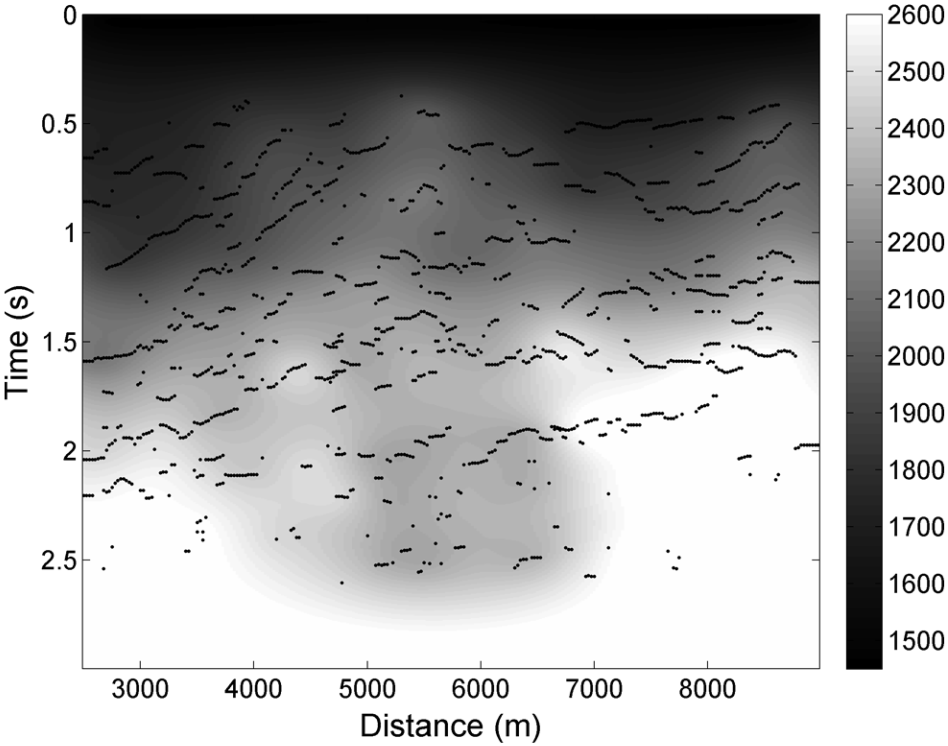
\includegraphics[scale=.16]{7a.png}
    }
    \subfigure[迭后记录. \label{fig:7b}]{
        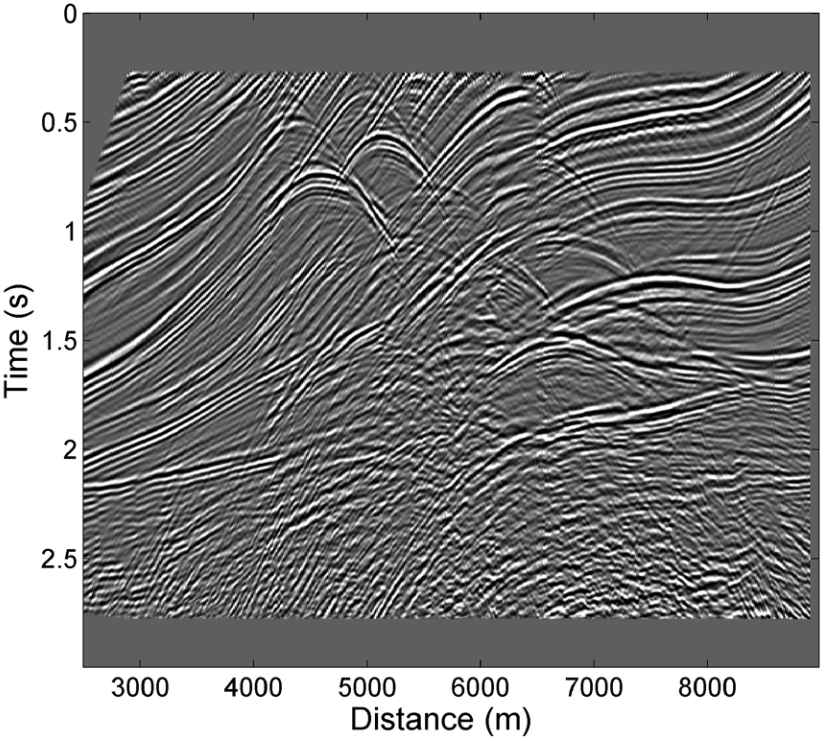
\includegraphics[scale=.16]{7b.png}
    }
    \caption{估计的叠加速度模型和迭后记录. \label{fig:7}}
\end{figure}
图~\ref{fig:7a} 是用这些结点插值得到的叠加速度, 最终的结点速度位置在速度模型上用黑点标记. 有了图~\ref{fig:6a} 中CMP位置相应的NMO速度, 便可以进行NMO了, 其结果如图~\ref{fig:6c} 所示. 可以看出道集已经成功被拉直了. 在对所有CMP道集进行处理后, 通过沿偏移方向累加得到图~\ref{fig:7b} 中的迭后记录, 主反射事件是连续的, 衍射在迭后记录上是清晰的, 这证实了叠加速度模型的有效性. 
\begin{figure}[htb]
    \centering
    \subfigure[整个数据集的插值速度模型. \label{fig:8a}]{
        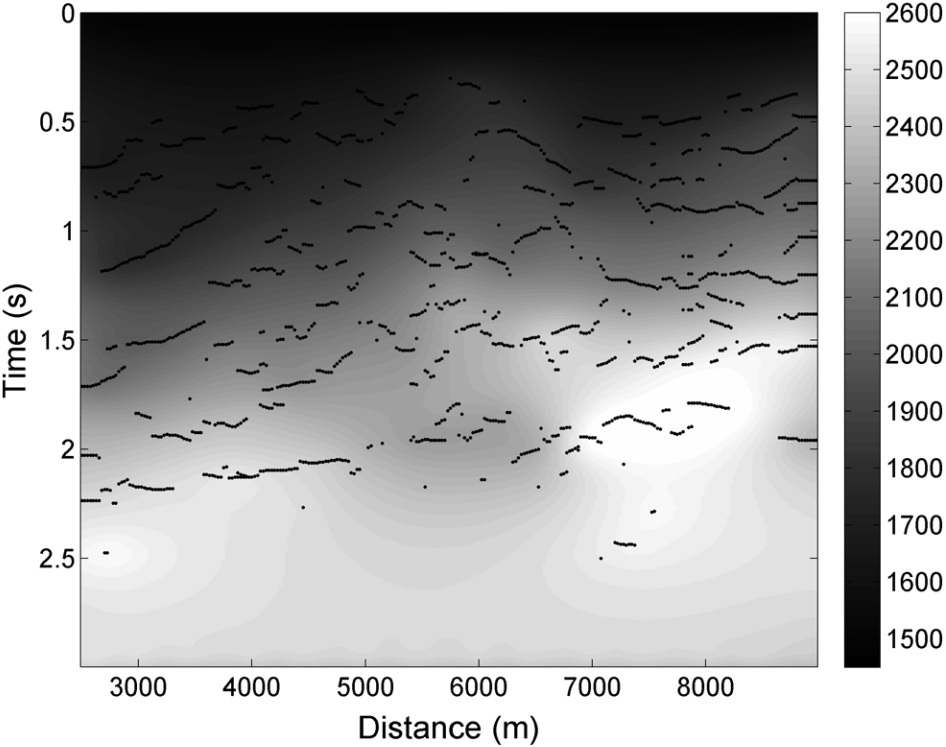
\includegraphics[scale=.16]{8a.png}
    }
    \subfigure[迭前Kirchhoff时偏移的迭后记录. \label{fig:8b}]{
        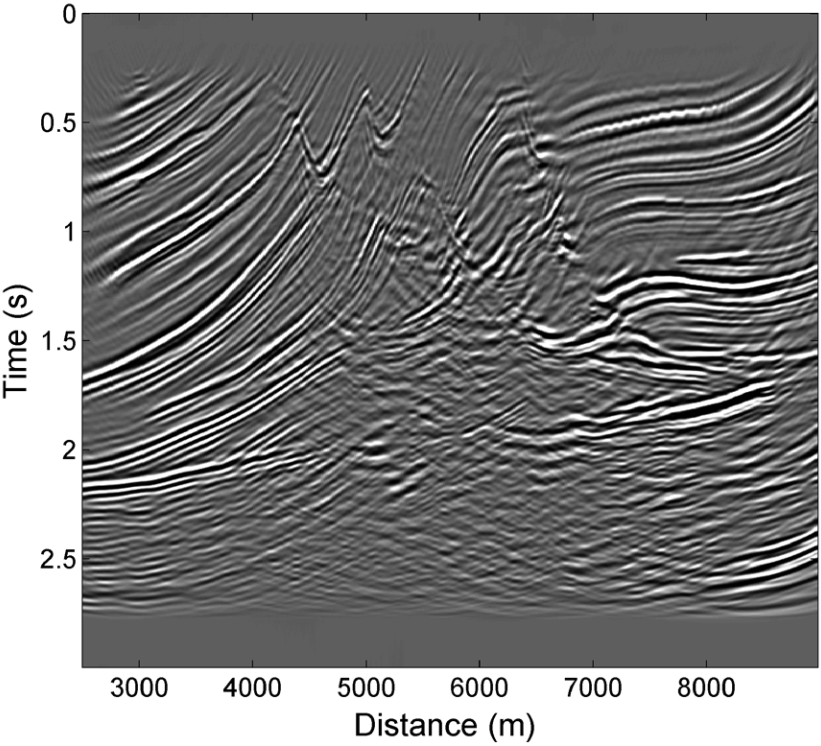
\includegraphics[scale=.16]{8b.png}
    }
    \caption{迭前时偏移速度估计模型和估计的迭前Kirchhoff时偏移. \label{fig:8}}
\end{figure}

有了来自两个不同道集的局部同相轴斜率$p_h, p_y$, 我们就可以直接映射得到与时偏移相关的局部属性. 我们需要做的就是将迭前空间$\{t,h,y\}$中的数据点映射到时偏移图像空间$\{\tau,x,V_{\mathrm{mig}}\}$. 以新空间中的局部属性作为输入, 用加速密度聚类算法进行自动时偏移速度估计. 利用速度不确定度约束选取每个CIG上的结点时偏移速度. 最终得到的时偏移速度在图~\ref{fig:8a} 中被标记为黑点. 利用插值时偏移速度模型, 可以得到迭前Kirchhoff时偏移. 图~\ref{fig:8b} 为迭前Kirchhoff偏移的叠加部分. Marmousi模型中间部分的主要断层成像良好, 虽然Kirchhoff偏移的涂抹效应引起的偏移噪声仍然存在, 但偏移断面揭示了地下的主要结构, 这证实了时偏移速度模型的有效性. 
\subsection{实际数据集}
为了验证所提出的方法在真实地震数据上的性能, 我们选择了马达加斯加包(Madagascar package, \cite{Fomel2013})中提供的墨西哥湾历史数据集(Mexico data set, \cite{Claerbout1995}). 实际数据最初是储存在CMP道集中. 为方便起见, 我们用PWD分别估计CMP上的局部同相轴斜率$p_h, p_y$和共偏道集. 只需要CMP上的局部同相轴斜率$p_h$来得到NMO的局部属性. 由于地下结构比较简单, 因此速度不确定度设置为$10\%$. 
\begin{figure*}
    \centering
    \subfigure[单个CMP道集. \label{fig:9a}]{
        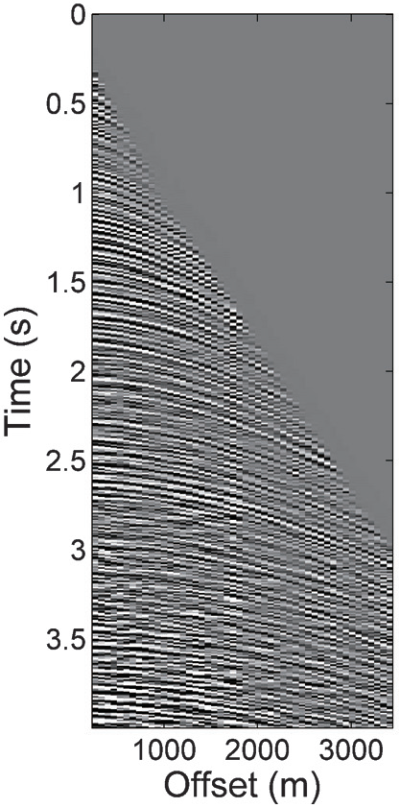
\includegraphics[scale=.33]{9a.png}
    }
    \subfigure[由直方图函数计算出的近似聚类中心. \label{fig:9b}]{
        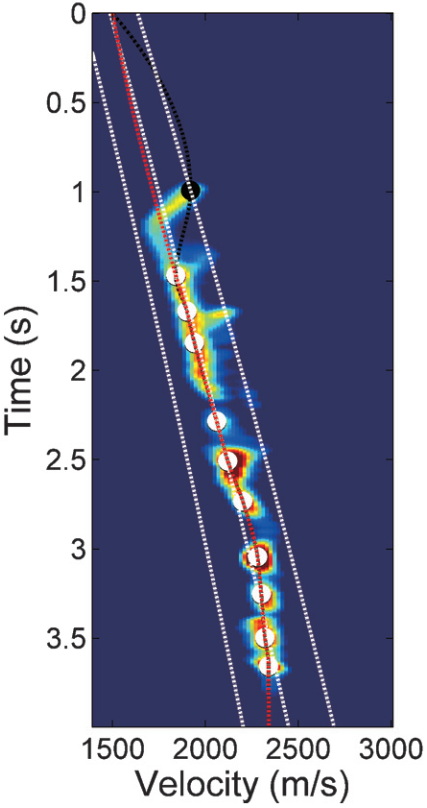
\includegraphics[scale=.33]{9b.png}
    }
    \subfigure[NMO校正后的道集与自动估计的叠加速度. \label{fig:9c}]{
        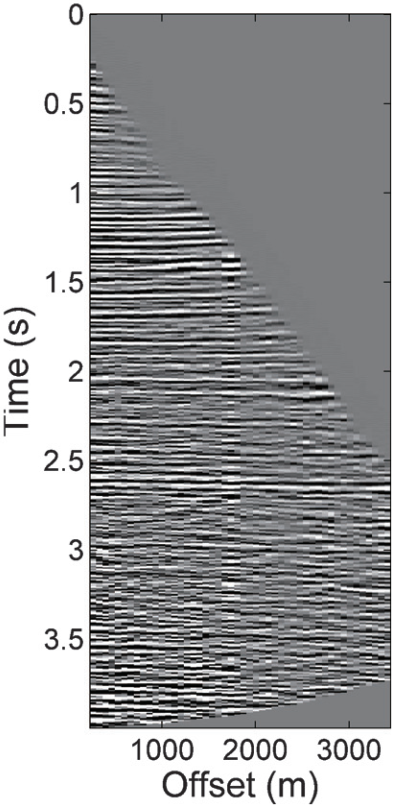
\includegraphics[scale=.33]{9c.png}
    }
    \caption{在单个CMP道集的实际数据上提取的结点速度. 二阶多项式函数拟合的NMO速度和速度不确定度上下界在面板~\ref{sub@fig:9a} 中用白色虚线标出. 超出速度不确定度的聚类速度结被去掉, 为黑色圆圈. 黑色虚线描述的是所有聚类中心的初始立方B-splines插值速度, 红色虚线显示的是过滤后的聚类中心的立方B-splines插值速度, 标记为白色圆圈. \label{fig:9}}
\end{figure*}

图~\ref{fig:9a} 显示了勘测线上10.72公里处的CMP道集情况. 如图~\ref{fig:9b} 所示, 以映射后的局部属性为数据点, 用直方图函数估计局部密度, 加速密度聚类算法中的近似聚类中心用白色和黑色圆圈标记, 多项式拟合的NMO速度和速度不确定度用白色虚线标记. 超过速度不确定度界限的聚类速度结被去掉, 被表示为黑圆圈. 图~\ref{fig:9b} 中的黑色虚线描述了所有聚类中心的初始插值速度, 红色虚线显示的是过滤后的聚类中心的插值速度, 标记为白色圆圈, 基于这些直方图上过滤后的聚类中心, 我们用原始数据集更新聚类中心. 有了CMP位置相应的NMO速度, 可以对道集进行NMO校正, 其结果如图~\ref{fig:9c} 所示. 在此速度下, 道集已被成功地拉直. 
\begin{figure}[htb]
    \centering
    \subfigure[整个实际数据集的插值速度模型. \label{fig:10a}]{
        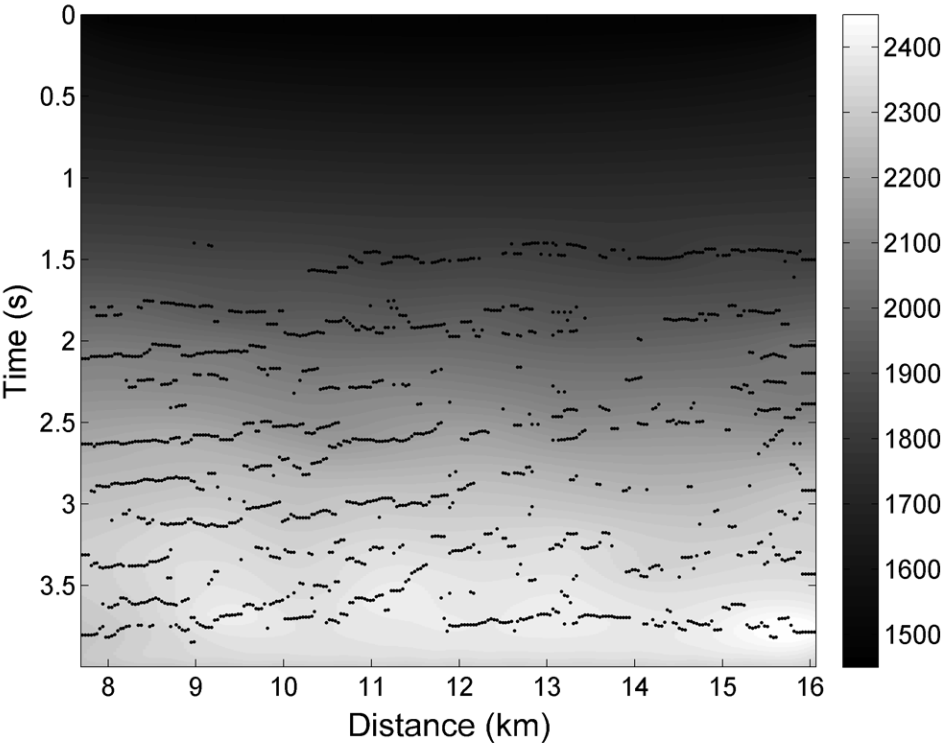
\includegraphics[scale=.16]{10a.png}
    }
    \subfigure[迭后记录. \label{fig:10b}]{
        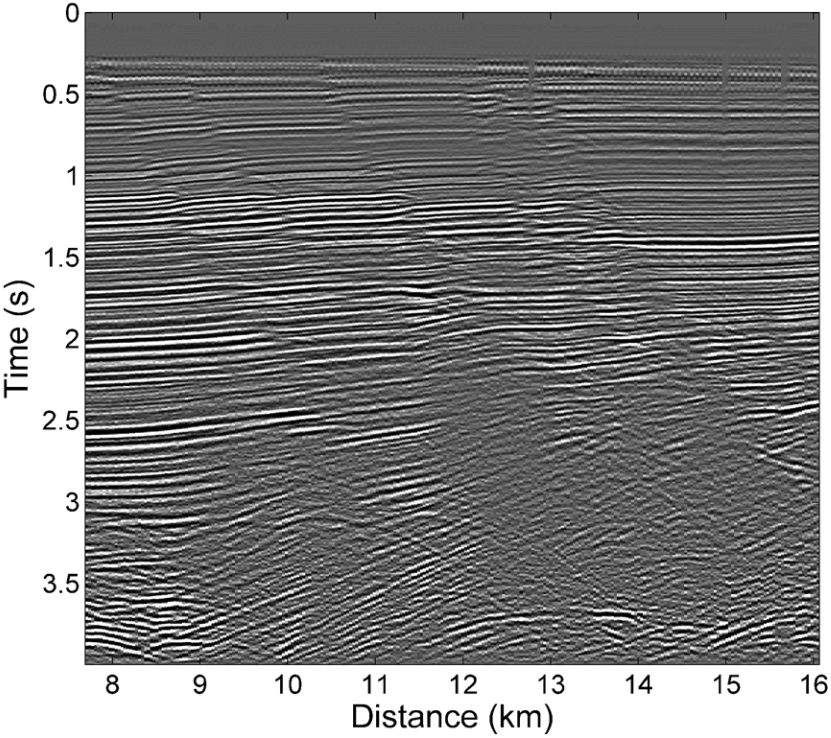
\includegraphics[scale=.16]{10b.png}
    }
    \caption{估计出的叠加速度模型和实际数据集的迭后记录. \label{fig:10}}
\end{figure}
估计出的整个事件的叠加速度模型如图~\ref{fig:10a} 所示, 最终的结点叠加速度被标记为黑点. 相应的叠加断面如图~\ref{fig:10b} 所示, 可以看到, 主反射事件是连续的, 其衍射在断层区附近是十分清晰的. 
\begin{figure}[htb]
    \centering
    \subfigure[整个实际数据集的插值速度模型. \label{fig:11a}]{
        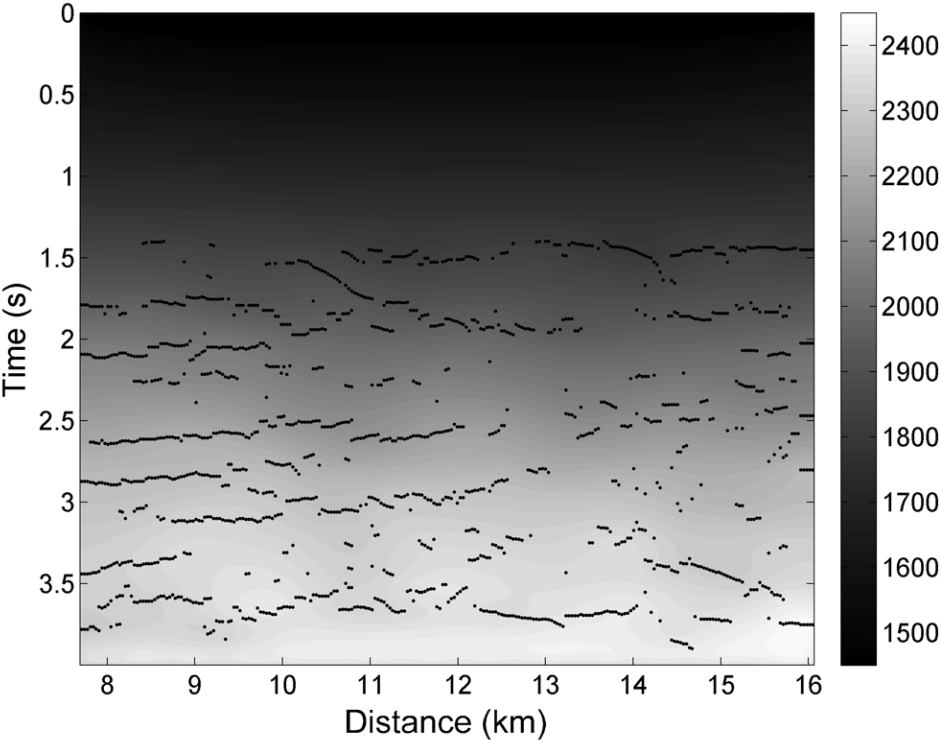
\includegraphics[scale=.16]{11a.png}
    }
    \subfigure[迭后记录. \label{fig:11b}]{
        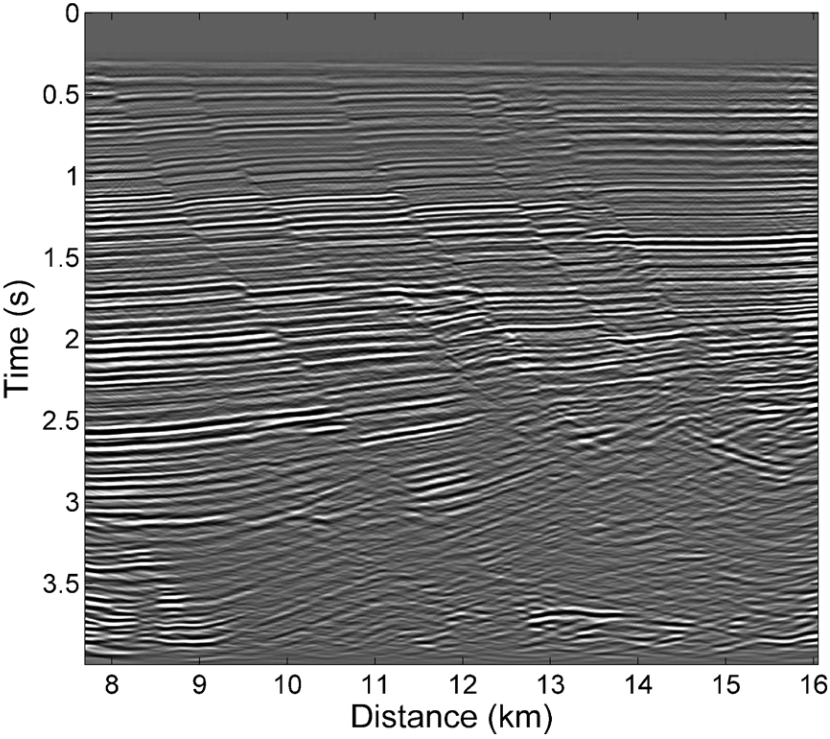
\includegraphics[scale=.16]{11b.png}
    }
    \caption{估计出的叠加速度模型和实际数据集的迭后记录. \label{fig:11}}
\end{figure}

实施时偏移速度估计, 需要局部同相轴斜率$p_h, p_y$. 如图~\ref{fig:11a} 所示, 迭前时偏移速度模型是通过插值建立的, 最终的结点时偏移速度标记为黑点. 用这个速度模型, 我们对整个数据集实施了迭前Kirchhoff时偏移. 图~\ref{fig:11b} 显示了每个共偏道集上的迭前Kirchhoff偏移的迭后记录. 很明显, 连续层和主要的断层都成像得很好. 冲突事件得到了合适的处理, 断层得到了正确的还原, 深层区域也得到了清晰的成像. 这些都证实了加速密度聚类算法进行自动速度估计的有效性. 同时, 该算法的计算效率较高, 因此有很大可能将其扩展到三维情况. 


